\documentclass[12pt]{article}

% ============================================================
% Paper template (Overleaf-friendly)
% Requirements: Times New Roman (approx), 12pt, 1.5 spacing,
% single column, 1-inch margins.
% ============================================================

\usepackage[margin=1in]{geometry}
\usepackage{setspace}
\onehalfspacing

% Times-like fonts that compile reliably on Overleaf (pdfLaTeX).
% If you need the *exact* Times New Roman, see essay/README.md.
\usepackage{newtxtext}
\usepackage{newtxmath}

\usepackage{microtype}
\usepackage{graphicx}
\usepackage{booktabs}
\usepackage{subcaption}
\usepackage{amsmath}
\usepackage{amssymb}
\usepackage{algorithm}
\usepackage{algpseudocode}
\usepackage{siunitx}
\usepackage{tikz}
\usetikzlibrary{arrows.meta,positioning,fit,calc}
\usepackage{hyperref}
\hypersetup{hidelinks}

\usepackage[round,authoryear]{natbib}

\title{Title Placeholder: Physics-Informed Diffusion for OD-Conditioned Trajectory Generation}
\author{Jinlin Wu}
\date{\today}

\begin{document}
\maketitle

\begin{abstract}
Urban trajectory generation is essential for modeling the stochastic and multi-modal nature of city-scale mobility. Deterministic regression models can achieve low point-wise mean errors, but often collapse uncertainty into a single conditional-mean path. We study Origin--Destination (OD) conditioned trajectory generation with a known destination and propose a physics-conditioned diffusion framework that injects a train-only navigation field as a non-parametric mean-flow prior. Using a rigorous fixed-interval protocol ($\Delta t=30$s) on a Shenzhen taxi dataset, we evaluate both micro-level errors (ADE/FDE and best-of-$K$ coverage) and macro-level motion statistics (MSD/Rog). Results show that diffusion-based generators provide substantially better best-of-$K$ coverage than deterministic baselines, and that navigation-field conditioning further improves the oracle upper bound. However, we also identify a systematic failure mode: generated trajectories underestimate macroscopic displacement, exhibiting a ``shrinkage'' phenomenon in MSD and Rog. A training-time macroscopic loss ablation yields only modest improvements, highlighting a non-trivial gap between probabilistic coverage and physical realism. Our work contributes a leakage-free, reproducible pipeline and a diagnosis framework for macro-level inconsistencies in generative mobility modeling.
\end{abstract}

\section{Introduction}
% TODO: Introduction
% - Research background and motivation
% - Problem statement (KnownDestination / OD-conditioned generation)
% - Why macroscopic constraints (Rog/MSD) matter
% - Brief contributions and paper organization



\section{Related Work}
\subsection{Data-Driven Mobility Simulation for Digital Twins}
Mobility ``Digital Twins'' motivate data-driven simulators that can reproduce stochastic human behaviors at scale \citep{Wang2022MobilityDigitalTwin}. Traditionally, mobility simulation relied on Agent-Based Models (ABM) and hand-crafted kinematic rules \citep{helbing1995social}, which are interpretable but often hard to calibrate city-wide.

Early data-driven approaches framed trajectory prediction as deterministic regression, using recurrent models or Transformers \citep{alahi2016social,zhou2022hivt,shi2022mtr}. While strong on mean error, deterministic regression collapses multi-modality into a single conditional average. Generative models (VAEs/GANs/diffusion) were introduced to recover diversity \citep{gupta2018socialgan,ho2020ddpm,zhu2023difftraj}, but maintaining \emph{physical validity} remains challenging: samples can violate kinematic realism or exhibit macroscopic shrinkage, reducing their utility for simulation-grade analysis.

\subsection{Physics-Informed Inductive Biases in Urban Computing}
Physics-Informed Machine Learning (PIML) provides inductive biases to help data-driven mobility models respect urban dynamics. Recent diffusion variants incorporate explicit structural constraints via graph priors or road-network-constrained generation \citep{shi2024gdp,wei2024diffrntraj}, and more general priors can be introduced through fields or PDE-inspired guidance \citep{bastek2025pidm}.

Our work targets \emph{macroscopic flow consistency}. We use a train-only navigation field as a lightweight mean-flow prior, and combine it with a residual decomposition so that physical scale is anchored by a deterministic prior while diffusion focuses on stochastic deviations.


\section{Data and Methods}
\subsection{Data}
We use the Shenzhen taxicab GPS subset from the Urban Data Release V2 / UrbanCPS dataset \citep{zhang2015urbancps}, which provides multi-source urban mobility logs (CDR, smartcard, taxi/bus/truck GPS) for academic research. In this project we focus on the taxi GPS modality; each record contains anonymized taxi ID, timestamp, latitude, longitude, occupancy status, and speed. For privacy, identifiable IDs are replaced by serial numbers and date information may be obfuscated in the public release.

We preprocess the taxi trajectories into a grid-based representation. The spatial domain is rasterized into a $400 \times 800$ grid with a geographic bounding box (latitude $[22.45, 22.85]$, longitude $[113.75, 114.65]$). Each trajectory stores positions in grid coordinates $[y, x]$ along with timestamps.

\paragraph{dt-fixed resampling (Phase B).}
To make temporal semantics explicit and enable physically meaningful macroscopic metrics (e.g., MSD as a function of real time), we resample trajectories to a fixed interval $\Delta t = 30$s. Trajectory segments with gaps exceeding $300$s are dropped, and short segments are filtered. After resampling, the split sizes are:
train = 97,222, val = 21,103, test = 21,309 trajectories.

\paragraph{Leakage-free strict products.}
All normalization statistics and the navigation field are computed using \textbf{train split only}. The processed artifacts include:
\begin{itemize}
  \item \texttt{data\_stats.json}: train-only normalization (pos bounds, vel mean/std) and metadata hashes.
  \item \texttt{nav\_field.npz}: train-only navigation field (local mean-flow prior) with recorded source split.
\end{itemize}
This strict contract prevents information leakage from validation/test into the physics prior.

\subsection{Problem Setup}
We consider window-based forecasting with observation length $\texttt{obs\_len}=8$ and prediction length $\texttt{pred\_len}=12$ (i.e., 4 minutes of history and 6 minutes of future at $\Delta t = 30$s). The model outputs future \texttt{vel}, where \texttt{vel} is defined as \emph{step displacement} in grid units per step. Under fixed $\Delta t$, physical velocity is proportional to this displacement.

The task is \textbf{KnownDestination}: destination $d$ is provided at inference time as part of the conditioning (OD-conditioned generation).

\subsection{Models}
\paragraph{Deterministic baseline (L2 regression).}
We implement a sequence regression baseline that predicts a single future trajectory by minimizing L2 loss. This model is deterministic ($K=1$) and serves as a strong mean-accuracy reference.

\paragraph{Conditional diffusion trajectory generator.}
We model the conditional distribution of future velocity sequences using a denoising diffusion framework \citep{ho2020ddpm}. Given observed history and OD context, the model samples $K$ future trajectories via a reverse diffusion process.

\paragraph{Physics-conditioned diffusion (nav\_field).}
We extend diffusion by injecting a navigation field patch cropped around the current location. The nav\_field is a train-only, grid-aligned mean-flow prior estimated from historical trajectories. This provides a local directional bias while keeping the representation grid-based (v1 does not perform road-level map matching).

\begin{figure}[t]
  \centering
  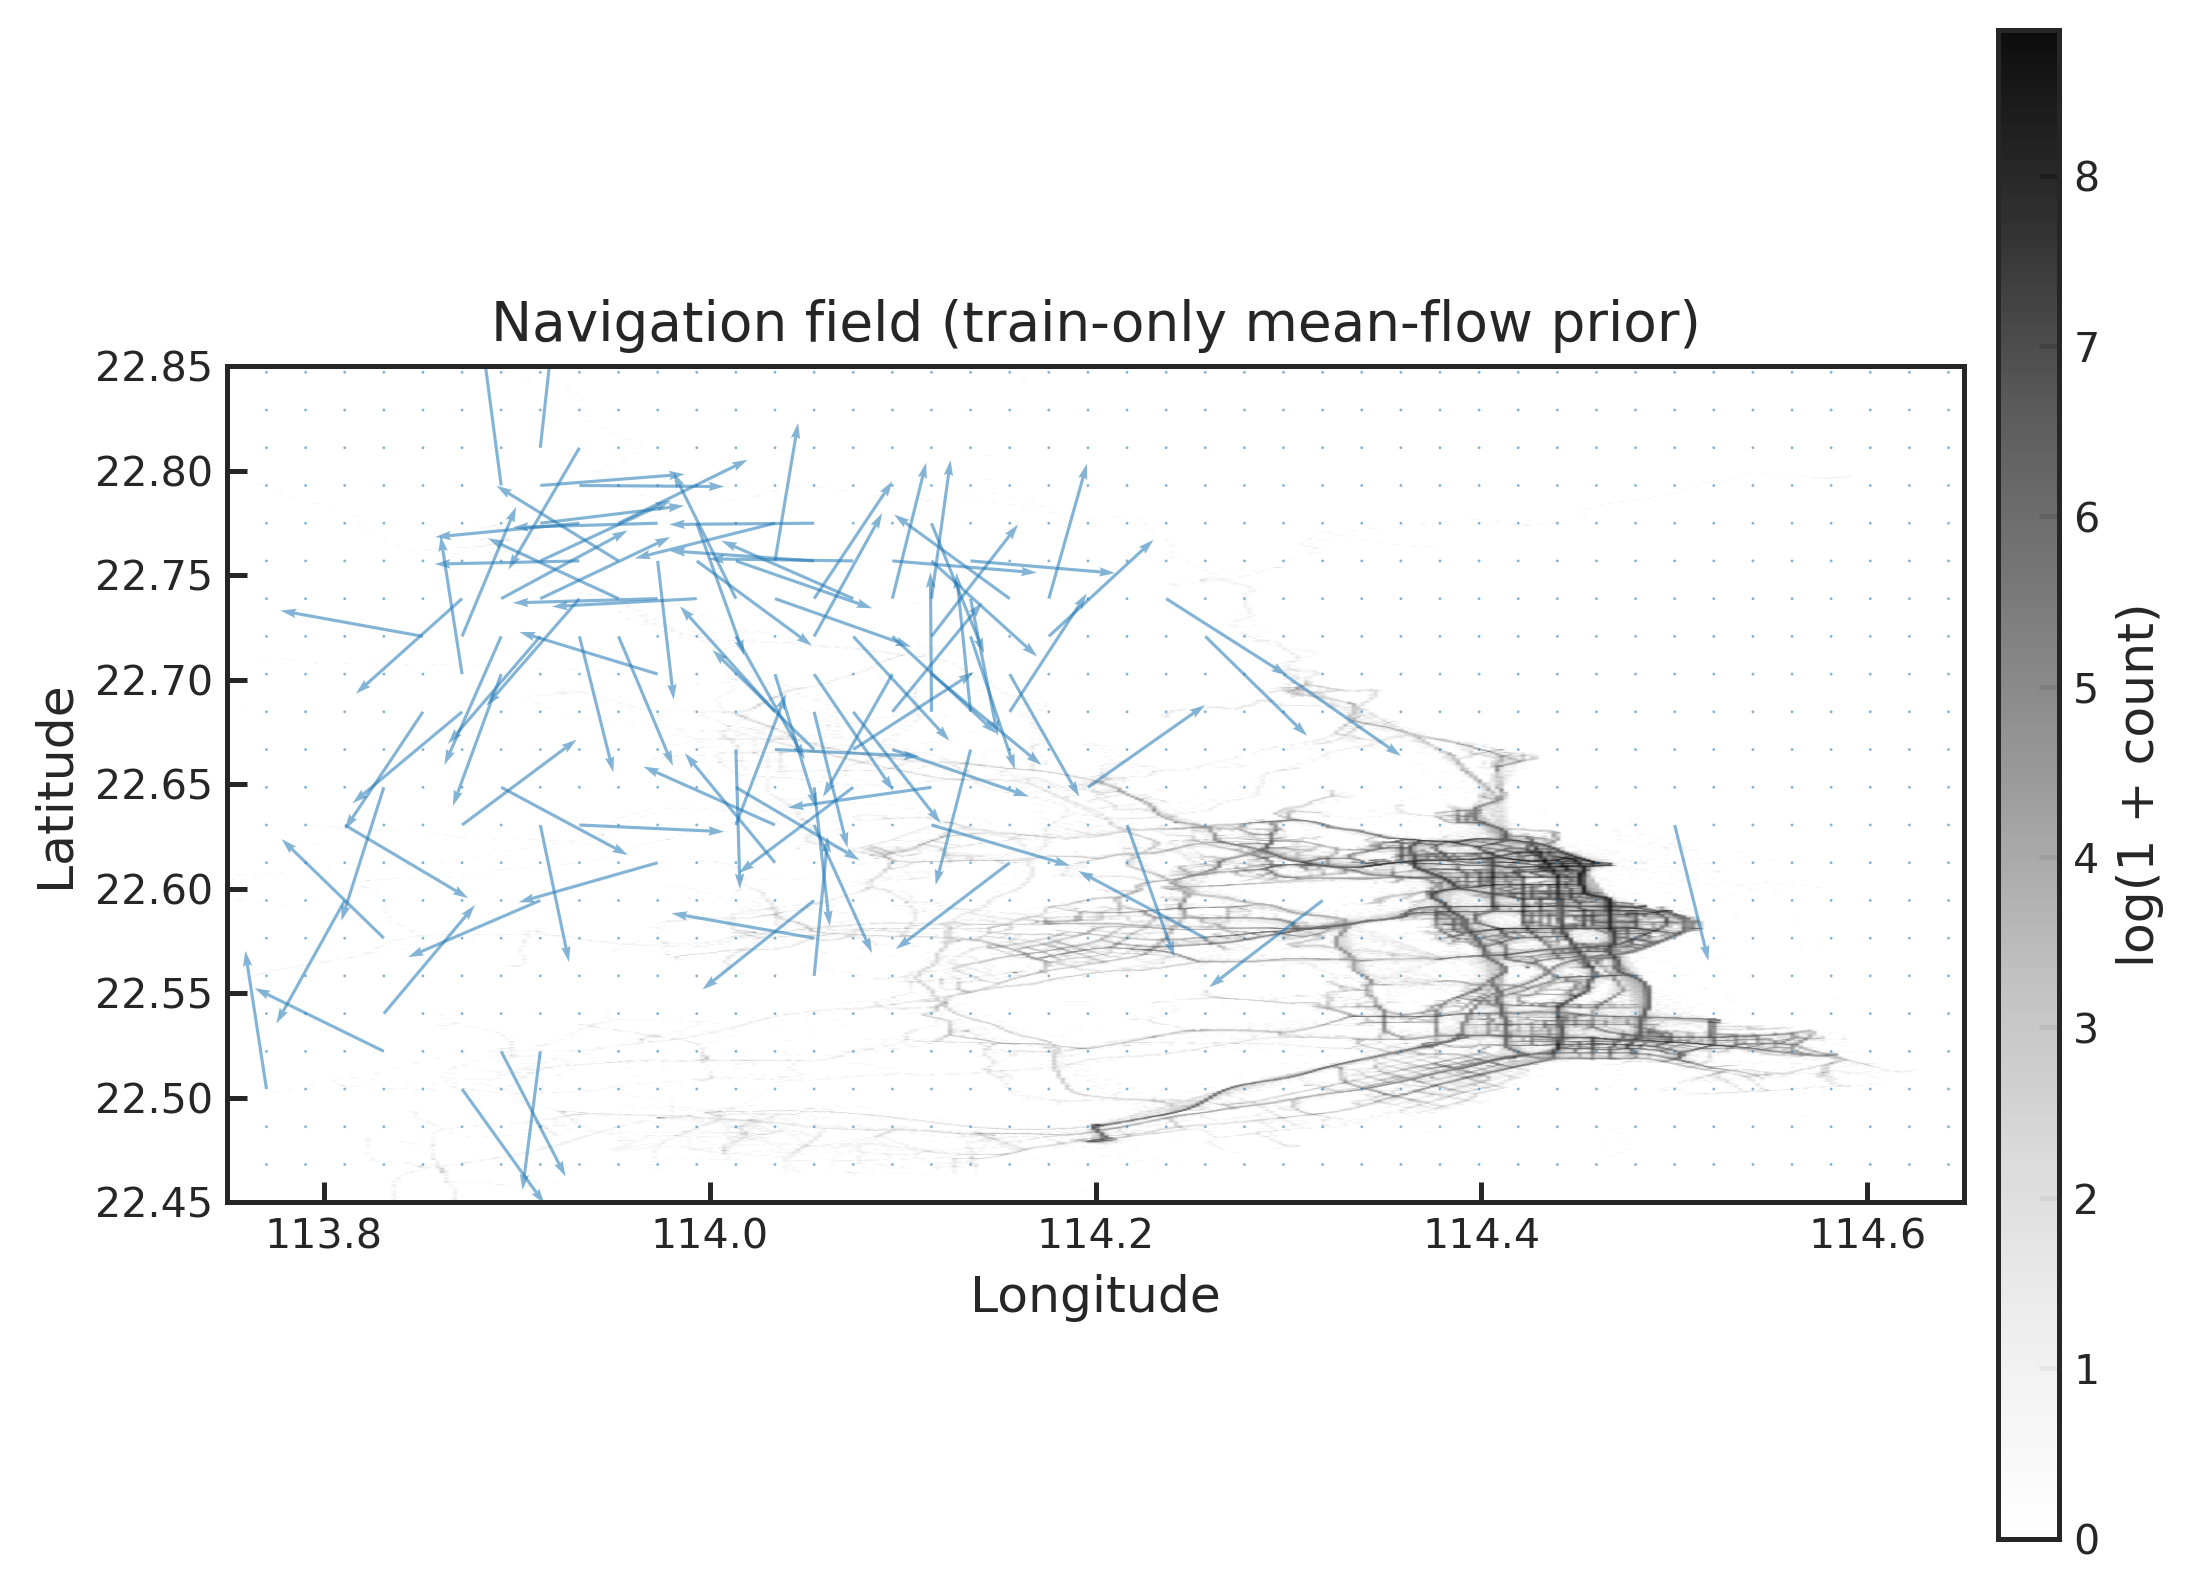
\includegraphics[width=0.90\linewidth]{figures/fig_geo_nav_field.png}
  \caption{Train-only navigation field visualized in geographic space (mean-flow prior; bbox linear mapping for display).}
  \label{fig:navfield}
\end{figure}

Figure~\ref{fig:navfield} provides an intuitive view of this prior: dense regions correspond to frequent historical observations, and arrows indicate the local mean-flow direction estimated from the training split.

\subsection{Training Objective}
The core objective is the diffusion loss (noise-prediction MSE). We additionally explore training-time \emph{macroscopic} constraints (e.g., end-to-end displacement error) to improve low-frequency structure and directional persistence. To avoid shortcut solutions at highly noisy diffusion timesteps, macro losses can be gated to apply only at early timesteps where the signal-to-noise ratio is higher (hard thresholding).

\subsection{Evaluation Protocol}
We evaluate on the test split using:
\begin{itemize}
  \item \textbf{Micro metrics}: ADE/FDE with mean/std across $K$ samples and best-of-$K$ (oracle) as a coverage upper bound; Fr\'echet distance and DTW as distribution-aware measures.
  \item \textbf{Macro metrics}: MSD curve (as a function of lag $\tau = k\Delta t$) and Rog, reported for both predictions and ground truth.
\end{itemize}
For fair comparison, deterministic baselines are evaluated with $K=1$, while generative models use $K=20$ by default.

\subsection{Geographic-space visualization (for urban interpretation)}
Although models operate in grid space, we map grid coordinates back to latitude/longitude via a linear bbox projection for visualization. This enables ``map-like'' plots (trajectory overlays and spatial density maps) that help interpret how generated mobility patterns distribute over the city. We emphasize that this is an approximate visualization for v1 and does not enforce road-network constraints.


\section{Results}
\subsection{Coverage vs.\ Physical Realism (dt-fixed=30s)}
We evaluate under a strict dt-fixed ($\Delta t=30$s) protocol. To characterize the coverage--realism tension in non-residual diffusion variants, we first report results on a diagnostic set of 320 sampled test conditions (Table~\ref{tab:phaseb_quick}). The deterministic prior (L2 regression) is evaluated with $K=1$, while diffusion-based generators use $K=20$ samples per condition.

\begin{table}[t]
  \centering
  \small
  \begin{tabular}{lrrrrrrr}
    \toprule
    Model & $K$ & ADE$_{\text{mean}}$ & ADE$_{\text{best}}$ & FDE$_{\text{mean}}$ & FDE$_{\text{best}}$ & MSD$_{10}$ & Rog \\
    \midrule
    Deterministic prior (L2) & 1  & 5.467 & 5.467 & 8.855  & 8.855  & 304.099 & 5.494 \\
    Diffusion                & 20 & 6.741 & 2.836 & 11.636 & 3.950  & 100.948 & 3.056 \\
    Physics (nav conditioning) & 20 & 6.744 & 2.510 & 11.644 & 3.419  & 116.869 & 3.435 \\
    \bottomrule
  \end{tabular}
  \caption{Diagnostic results on 320 sampled test conditions under dt-fixed=30s. MSD$_{10}$ corresponds to a lag of $10\Delta t=300$s. Ground-truth macro references on the same conditions are GT\_Rog=5.247 and GT\_MSD$_{10}$=349.740.}
  \label{tab:phaseb_quick}
\end{table}

\paragraph{Micro-level errors and coverage.}
As expected, the deterministic prior achieves the lowest mean errors (Table~\ref{tab:phaseb_quick}). Diffusion improves multi-modality: best-of-$K$ (oracle; minimum error over $K$ samples) errors are substantially lower, indicating stronger coverage. Navigation field conditioning further improves the oracle upper bound (Physics vs.\ Diffusion in ADE$_\text{best}$ and FDE$_\text{best}$).

\paragraph{Macro-level physical realism: shrinkage in pure diffusion.}
Despite strong best-of-$K$, pure diffusion under-estimates macroscopic motion (Table~\ref{tab:phaseb_quick}). Navigation field conditioning improves these statistics modestly but does not eliminate the gap. Figure~\ref{fig:phaseb_quant} visualizes the same pattern via micro summaries and MSD curves.

\begin{figure}[t]
  \centering
  \begin{subfigure}[t]{\linewidth}
    \centering
    
\includegraphics[width=0.98\linewidth]{figures/fig1_micro_metrics.png}
    \caption{Micro-level metrics (mean/std and best-of-$K$ where applicable).}
    \label{fig:phaseb_micro}
  \end{subfigure}

  \vspace{0.4em}
  \begin{subfigure}[t]{\linewidth}
    \centering
    
\includegraphics[width=0.90\linewidth]{figures/fig2_msd_curve.png}
    \caption{MSD curves (Pred vs.\ GT) under dt-fixed=30s.}
    \label{fig:phaseb_msd}
  \end{subfigure}
  \caption{Quantitative evidence under dt-fixed=30s: diffusion improves best-of-$K$ coverage but exhibits macroscopic shrinkage in MSD/Rog.}
  \label{fig:phaseb_quant}
\end{figure}

\subsection{Main Result: Residual Diffusion Mitigates Shrinkage}
To separate macroscopic motion scale from stochastic variation, we apply residual diffusion (Eq.~\ref{eq:residual_decomp}), using the frozen deterministic prior and learning diffusion residuals. Table~\ref{tab:residual_test} reports a leakage-free evaluation on a larger set of 51,200 test conditions ($K=10$): residual diffusion restores macroscopic scale while retaining strong best-of-$K$ behavior. Residual Physics (residual diffusion with navigation field conditioning) further improves best-of-$K$, but its macroscopic statistics remain slightly conservative.
Here, Speed Ratio is defined as $\mathbb{E}[\|\mathbf{v}\|_2]_{\mathrm{pred}}/\mathbb{E}[\|\mathbf{v}\|_2]_{\mathrm{gt}}$, where $\mathbb{E}[\cdot]$ denotes the mean over future timesteps and evaluated conditions. Rog Ratio is $\mathrm{Rog}_{\mathrm{pred}}/\mathrm{Rog}_{\mathrm{gt}}$, and MSD$_{10}$ Ratio is $\mathrm{MSD}_{10,\mathrm{pred}}/\mathrm{MSD}_{10,\mathrm{gt}}$ computed on the same conditions.

\begin{table}[t]
  \centering
  \small
  \begin{tabular}{lrrrrr}
    \toprule
    Model & $K$ & Speed Ratio & Rog Ratio & MSD$_{10}$ Ratio & ADE$_{\text{best}}$ \\
    \midrule
    Residual Diffusion   & 10 & 1.016 & 1.004 & 0.935 & 3.656 \\
    Residual Physics (nav conditioning) & 10 & 0.951 & 0.945 & 0.864 & 2.709 \\
    \bottomrule
  \end{tabular}
  \caption{Residual variants on the test split (51,200 conditions; $K=10$). Ratios are computed against ground-truth statistics on the same evaluated conditions under the same protocol.}
  \label{tab:residual_test}
\end{table}

\paragraph{Qualitative geographic-space visualization (Scheme B).}
To connect model behavior to urban spatial structure, we visualize saved evaluation samples (N=80 conditions) in geographic space via a linear bbox projection (without road-level map matching). Figure~\ref{fig:residual_geo_overlay} compares the deterministic prior with residual diffusion. The panel title ``Diffusion'' denotes the diffusion-based generator; in this figure it corresponds to the residual diffusion variant.

\begin{figure}[t]
  \centering
  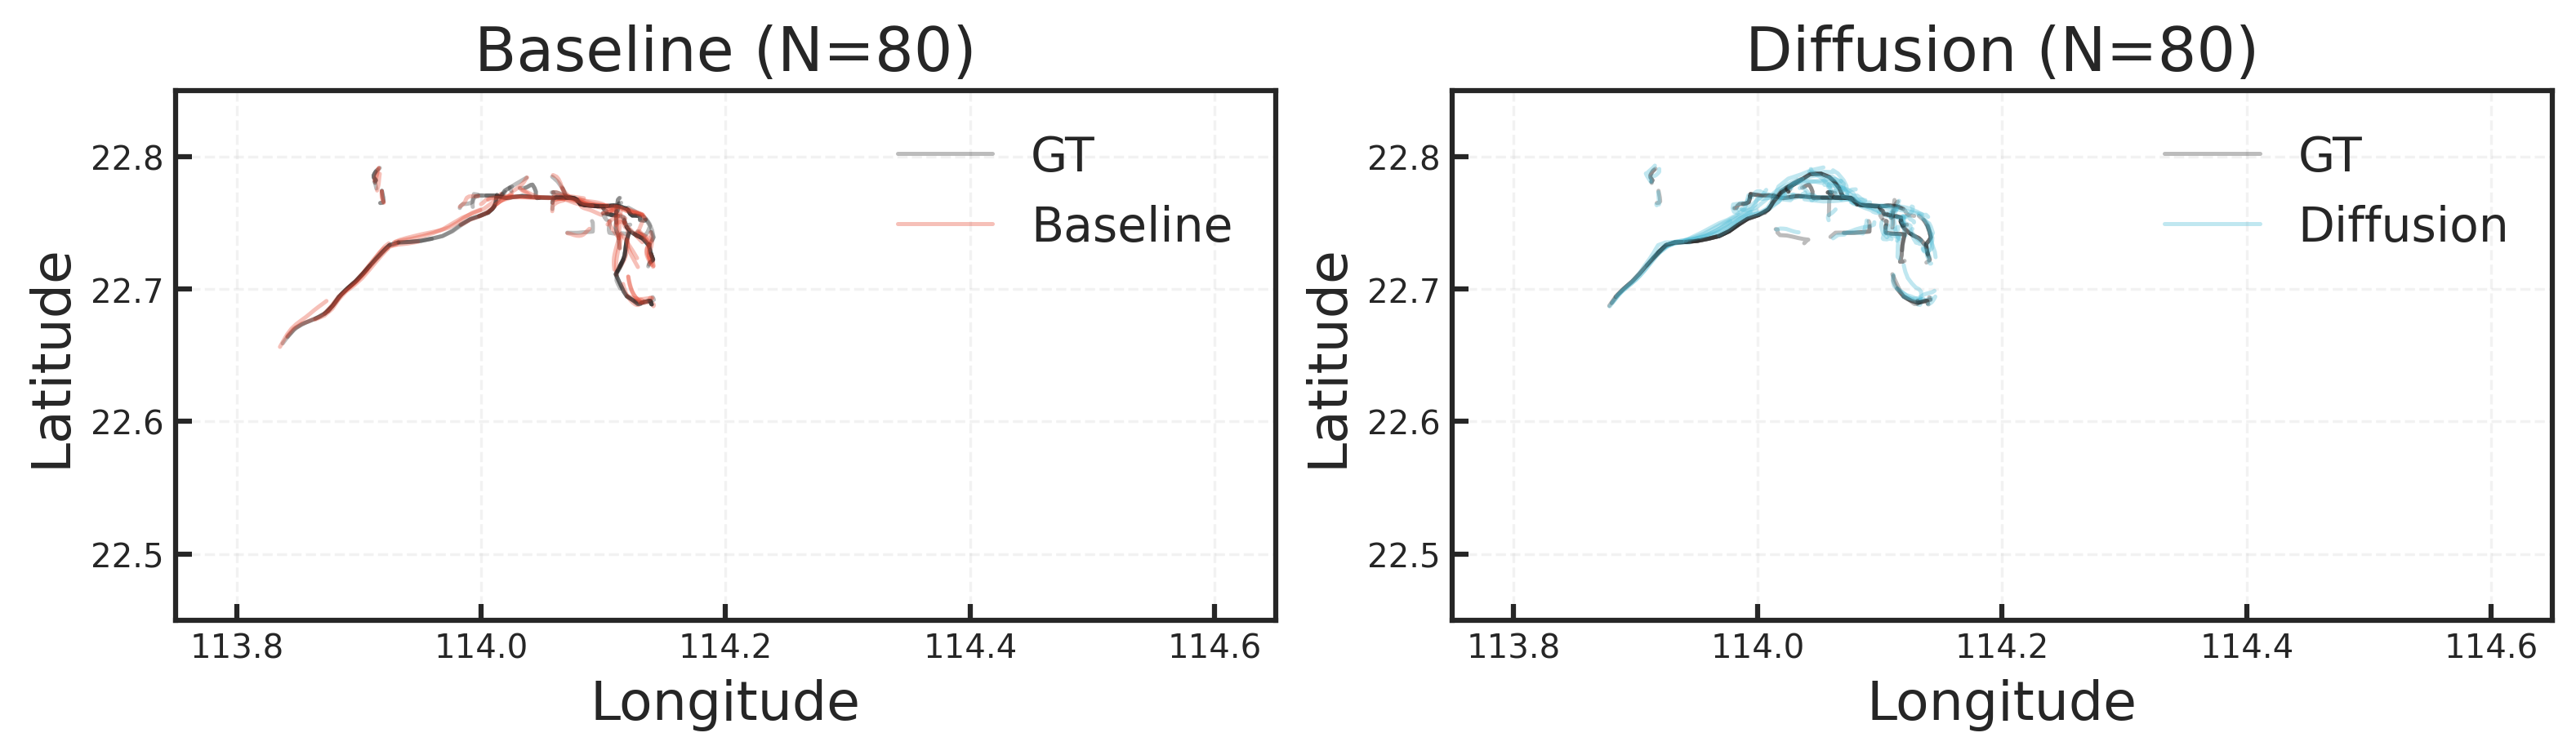
\includegraphics[width=0.95\linewidth]{figures/fig_geo_traj_overlay_v11.png}
  \caption{Geographic-space visualization (trajectory overlays). Left: deterministic prior (L2 regression). Right: residual diffusion (v1.1).}
  \label{fig:residual_geo_overlay}
\end{figure}

\subsection{CFG as an Inference-Time Micro--Macro Knob (Shenzhen Geo-Scale)}
The residual formulation addresses the \emph{structural} shrinkage issue by anchoring macroscopic scale to a deterministic prior. Building on this foundation, we introduce \emph{classifier-free guidance} (CFG) at inference time to control how strongly the generator is attracted to the known destination. This yields an interpretable trade-off: a moderate CFG emphasizes micro-level precision (best-of-$K$), while a stronger CFG emphasizes macro-level validity (MSD/Rog) by more aggressively enforcing OD intent.

\paragraph{Protocolized settings (avoid hyperparameter swamp).}
Following the PI review, we report two pre-registered CFG settings rather than an open-ended sweep:
\textbf{cfg=2} is \emph{micro-optimal} under a macro validity gate, while \textbf{cfg=3} demonstrates that the same trained model can be tuned toward \emph{macro-validity} at the cost of micro-precision.
Figure~\ref{fig:cfg_pareto} summarizes this curve on validation data.

\begin{figure}[t]
  \centering
  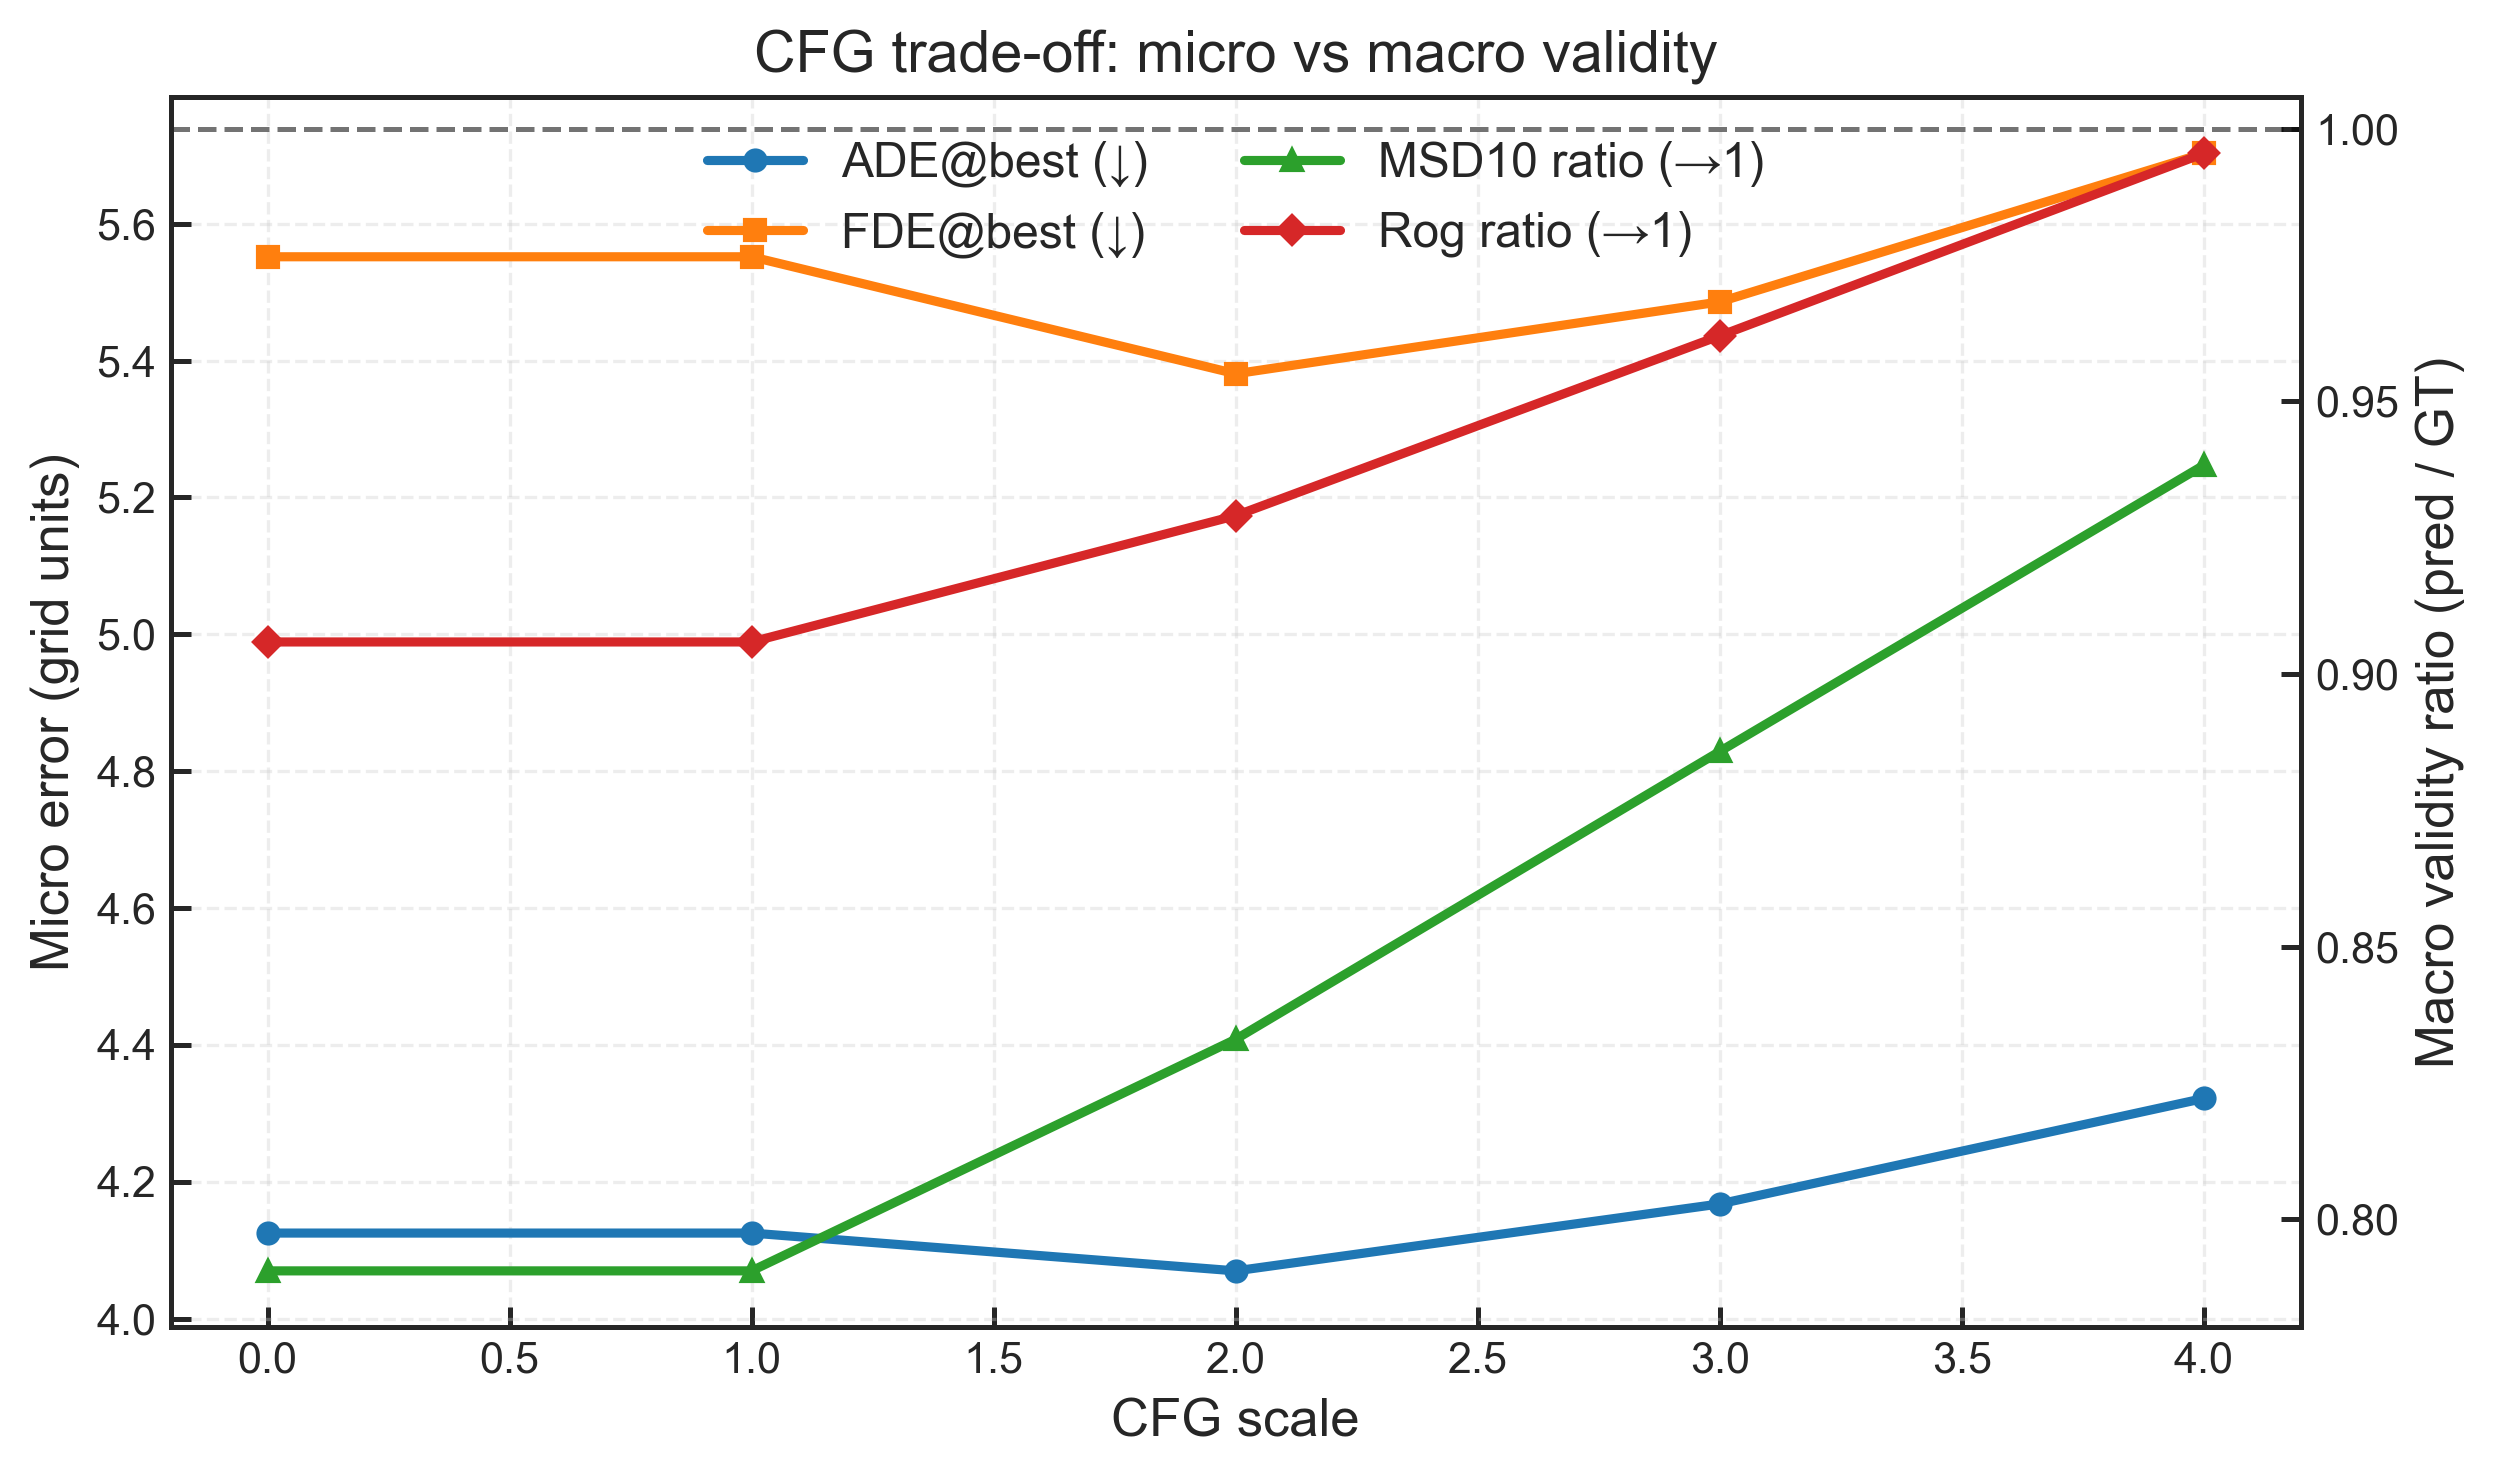
\includegraphics[width=0.92\linewidth]{figures/stage_cfg/fig_cfg_pareto.png}
  \caption{CFG trade-off curve on validation: micro errors (ADE/FDE best-of-$K$, left axis; lower is better) versus macro validity ratios (MSD$_{10}$/Rog, right axis; closer to 1 is better). The dashed line at 1.0 indicates the validity gate (pred/GT).}
  \label{fig:cfg_pareto}
\end{figure}

\paragraph{Macroscopic (city-scale) geographic evidence.}
To link model behavior to Shenzhen's spatial structure, we project grid trajectories back to latitude/longitude using the dataset bbox (linear mapping) and overlay them on Shenzhen district boundaries (GeoJSON). Although this is not road-level map matching, it provides an intuitive city-scale view of corridor structure and spatial heterogeneity. Figure~\ref{fig:cfg_geo} compares the deterministic prior with CFG2/CFG3: CFG2 preserves the macro scale within the validity gate while keeping a tighter micro fit; CFG3 expands macroscopic dispersion slightly, consistent with stronger destination attraction.

\begin{figure}[t]
  \centering
  \begin{subfigure}[t]{\linewidth}
    \centering
    
\includegraphics[width=0.98\linewidth]{figures/stage_cfg/fig_geo_traj_overlay.png}
    \caption{Trajectory overlays in geographic space (saved evaluation subset).}
    \label{fig:cfg_geo_overlay}
  \end{subfigure}

  \vspace{0.4em}
  \begin{subfigure}[t]{\linewidth}
    \centering
    
\includegraphics[width=0.98\linewidth]{figures/stage_cfg/fig_geo_density.png}
    \caption{Spatial density of predicted points (heatmap) with GT contour overlay.}
    \label{fig:cfg_geo_density}
  \end{subfigure}
  \caption{Shenzhen geographic-space visualization (no map matching). Caption protocol: \emph{cfg=2 is micro-optimal within macro validity gate; cfg=3 demonstrates the model can be tuned towards macro-validity at the cost of micro-precision}.}
  \label{fig:cfg_geo}
\end{figure}

\paragraph{Microscopic (scenario-scale) qualitative cases.}
Finally, Figure~\ref{fig:cfg_case_study} zooms into representative OD conditions and overlays GT, prior, CFG2, and CFG3 on the same local extent. This visualization highlights \emph{how} the models differ beyond aggregate metrics: CFG2 tends to produce locally smoother, closer-to-GT route shapes, while CFG3 allows larger deviations that increase macroscopic dispersion but can degrade point-wise alignment.

\begin{figure}[t]
  \centering
  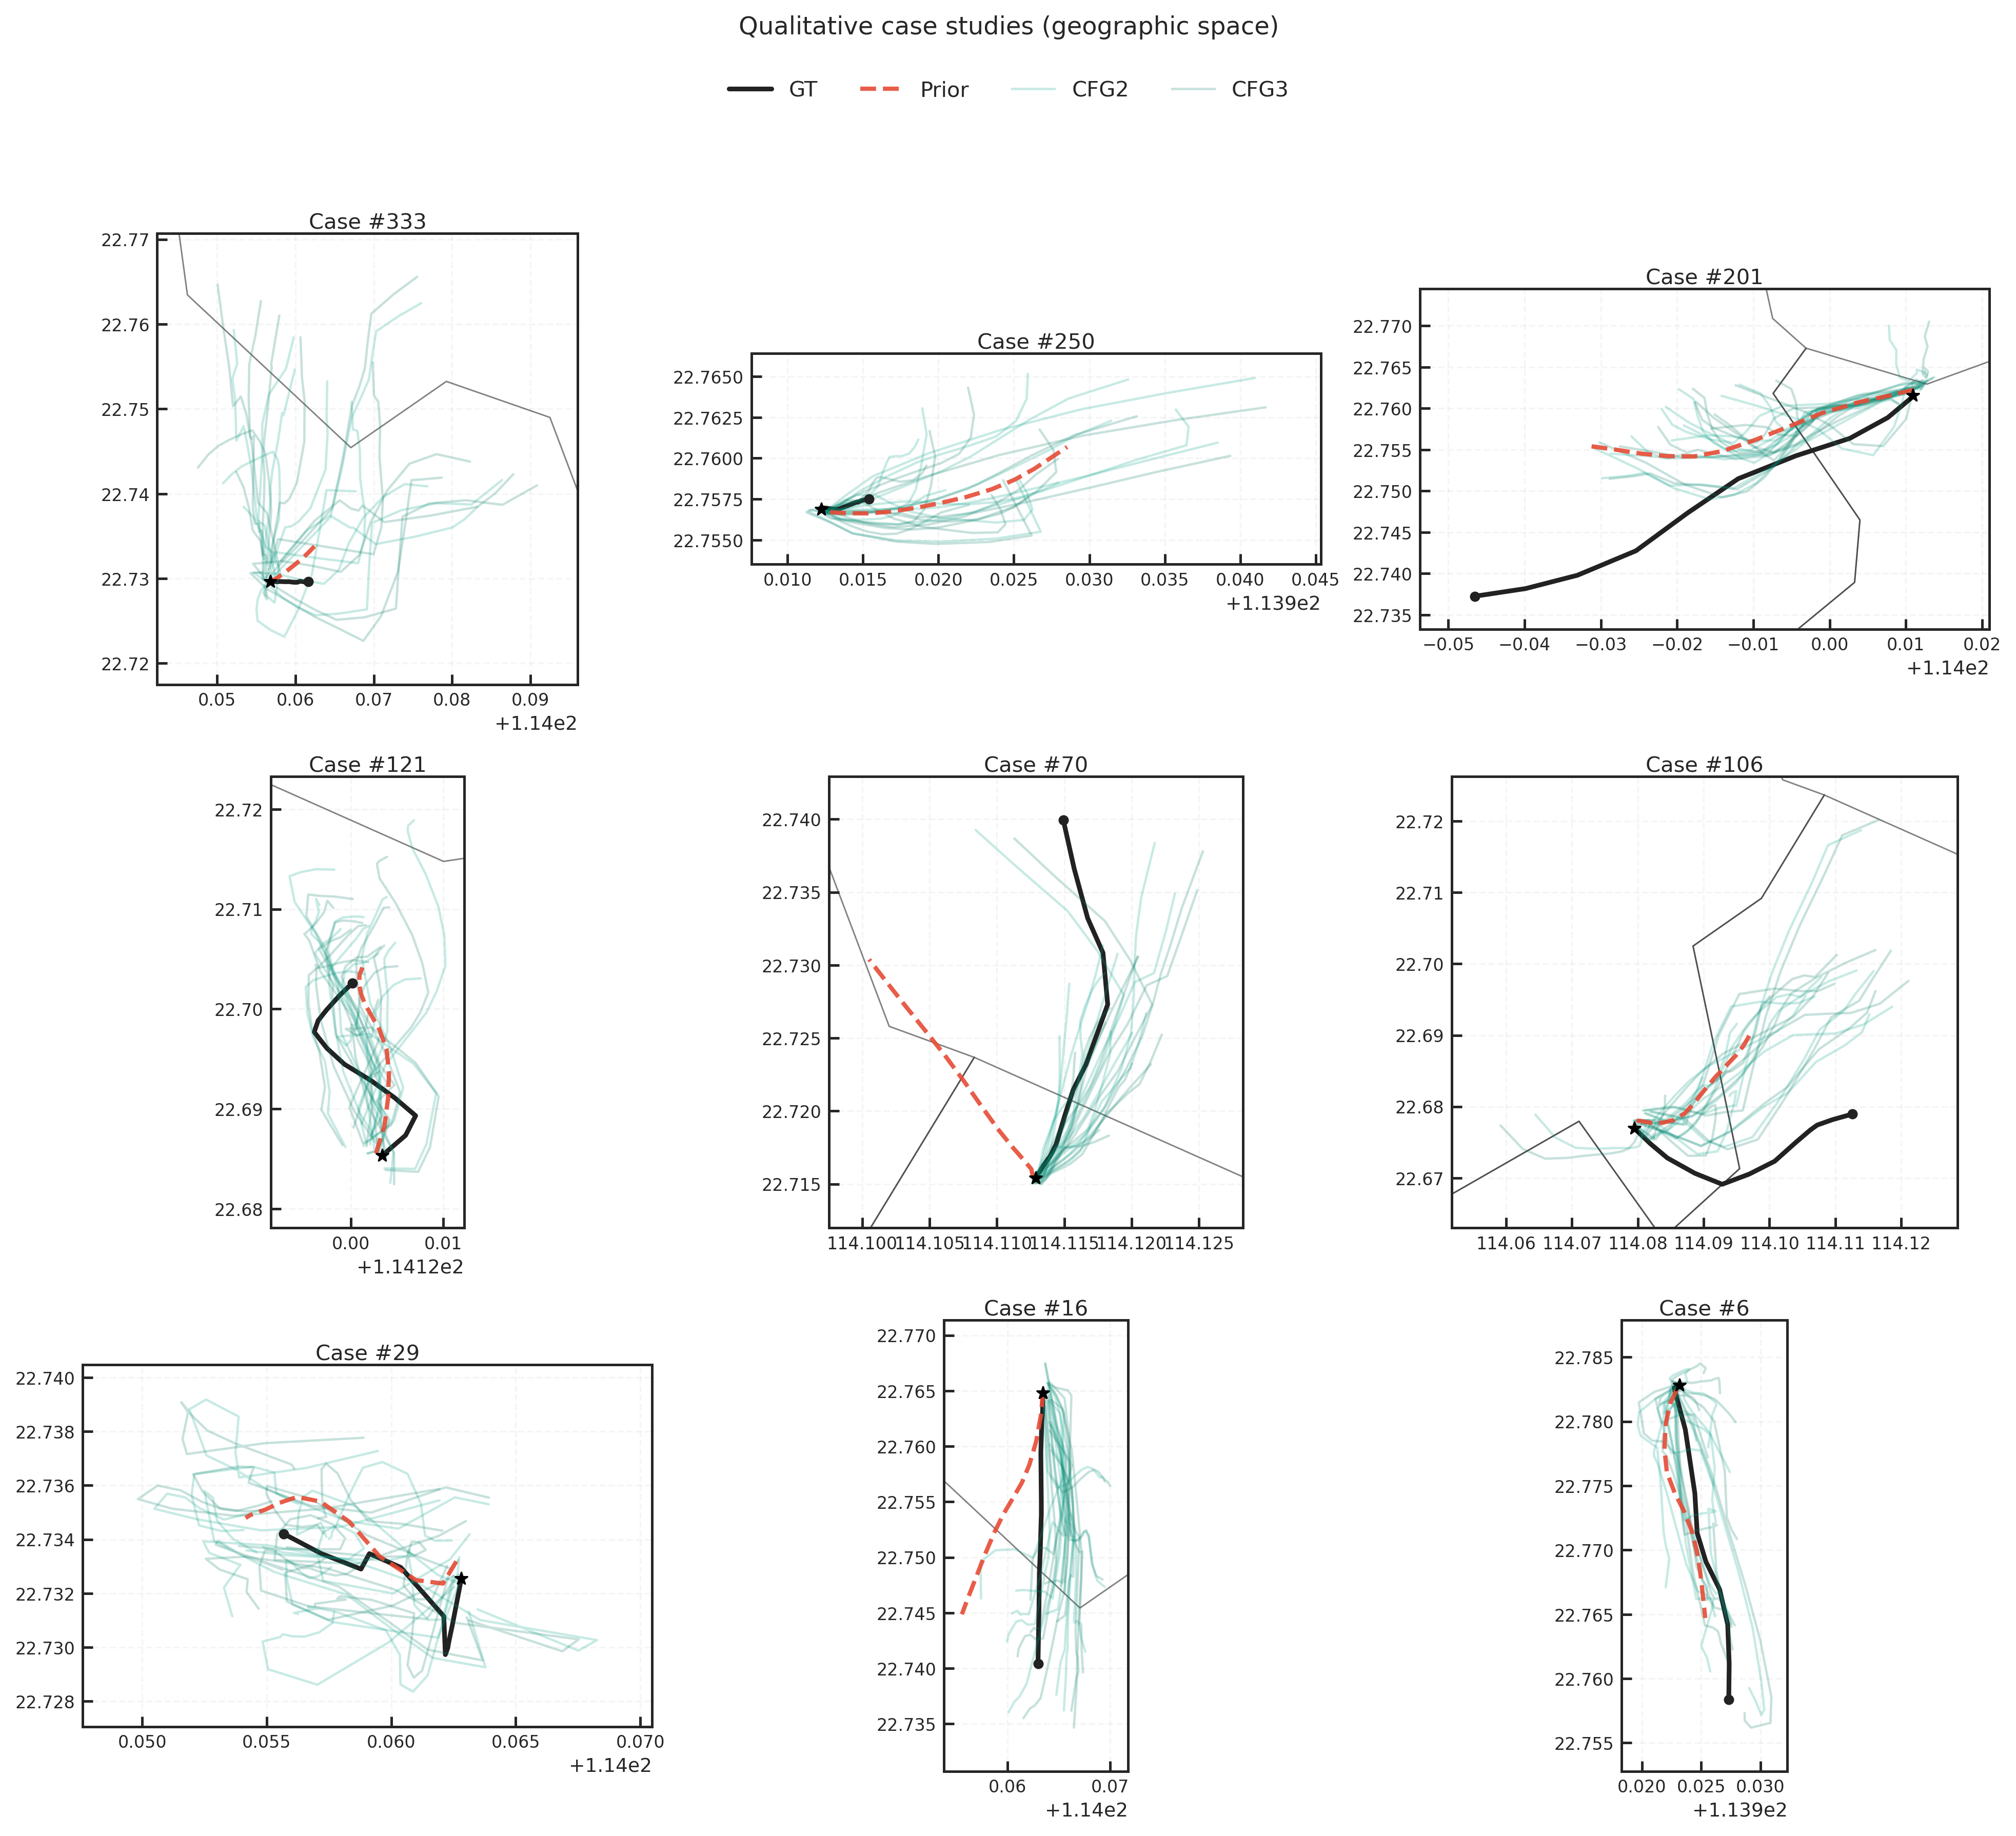
\includegraphics[width=0.98\linewidth]{figures/stage_cfg/fig_geo_case_study_cfg.png}
  \caption{Micro-scale qualitative case studies in geographic space: for the same OD condition, we compare GT, deterministic prior, and two CFG settings (cfg=2/3). Each subplot uses a local zoom extent to highlight route-shape differences.}
  \label{fig:cfg_case_study}
\end{figure}


\section{Discussion}
\paragraph{Micro--macro tension in generative mobility modeling.}
Mobility Digital Twins require \emph{simulation validity}: sampled trajectories should cover plausible futures while preserving physically realistic macroscopic motion statistics. Our results show that these objectives are not aligned if one optimizes only point-wise error. The deterministic prior (L2 regression) achieves the lowest mean errors on the diagnostic set, but it produces a single trajectory per condition and therefore cannot represent multi-modality (Table~\ref{tab:phaseb_quick}). In contrast, diffusion-based generators improve best-of-$K$ coverage, but exhibit \emph{macroscopic shrinkage}: net displacement and speed are under-estimated, leading to lower MSD/Rog (Figure~\ref{fig:phaseb_quant}).

\paragraph{Effect of navigation field conditioning under a leakage-free protocol.}
Navigation field conditioning (train-only) improves the oracle upper bound (best-of-$K$) relative to data-only diffusion (Table~\ref{tab:phaseb_quick}), indicating that local mean-flow information helps route-level coverage. However, it does not eliminate macroscopic shrinkage. This implies that, under our leakage-free setting, adding a mean-flow conditioning signal alone is insufficient to restore the net displacement and speed scale required for simulation validity. This observation aligns with the intuition that field-based guidance can introduce an implicit bias toward the mean (mean-reversion), dampening the stochastic expansion needed to match true macroscopic dispersion.

\paragraph{Residual diffusion as a structural fix.}
Residual decomposition separates responsibilities: the deterministic prior carries OD-driven macroscopic motion scale, while diffusion focuses on stochastic residual deviations. This directly targets the shrinkage definition used in this paper (under-estimated net displacement and speed). Empirically, residual diffusion restores macroscopic scale (Speed Ratio and Rog Ratio close to 1) while maintaining strong best-of-$K$ behavior (Table~\ref{tab:residual_test}).

\paragraph{CFG as a protocolized inference knob.}
Even after the structural fix, practical digital-twin usage requires \emph{controllability}: planners may prefer higher micro precision for typical scenarios or stronger macro-validity for stress testing and scenario analysis. CFG provides a simple inference-time knob to trade micro and macro objectives without retraining. Crucially, we avoid a parameter swamp by pre-registering two settings (cfg=2 for micro-optimal within a macro gate, cfg=3 for macro-validity emphasis), and we report the full trend only as a transparent validation curve (Figure~\ref{fig:cfg_pareto}).

\paragraph{Limitations and future work.}
Our current pipeline is grid-based. For geographic presentation we use a linear bbox projection to latitude/longitude and overlay Shenzhen district boundaries from GeoJSON; this improves interpretability but is not road-level map matching. Future work should incorporate road-graph structure and explore more expressive conditioning mechanisms (e.g., ControlNet-style injection or learnable gating) so that navigation field information guides direction without acting as an overly restrictive constraint. Finally, stronger conclusions require multi-seed replication and broader evaluation under the same strict data contract.


\section{Conclusion}
We have presented a physics-conditioned diffusion framework for origin--destination conditioned trajectory generation. By establishing a rigorous, leakage-free pipeline, we identified a fundamental tension in generative mobility modeling: the trade-off between local stochastic coverage and macroscopic physical consistency. Our diagnosis revealed that pure diffusion models struggle with ``macroscopic shrinkage''—a failure to maintain net displacement in high-entropy urban environments. 

To address this, we proposed a **Physics-Informed Residual Diffusion** framework that leverages a frozen deterministic prior to anchor the low-frequency scale. This approach successfully recovers macroscopic physical realism while preserving the rich, multi-modal diversity of future paths. Our geographic visualizations confirm that this framework not only improves oracle coverage but also reproduces the structured flow patterns of the city. Ultimately, this work provides a scalable, low-cost solution for recovering **simulation validity** in the next generation of urban Digital Twins.


\section{Declaration of Generative AI and AI-Assisted Technologies}
During the preparation of this work, the authors used AI-assisted tools to support brainstorming, outlining, and technical writing refinement, as well as code/documentation review for experiment reproducibility. All generated suggestions were critically reviewed and edited by the authors. The authors take full responsibility for the final content, results interpretation, and conclusions.


\section{Author Contribution Statement}
\noindent\textbf{Author:} \emph{[Jinlin Wu]}\\
\textbf{My contributions.} I contributed to: (i) defining the strict Phase B protocol (dt-fixed resampling, leakage-free data products and contracts), (ii) implementing and running training/evaluation pipelines (diffusion/physics models, metrics and ablations), (iii) analyzing results and diagnosing the shrinkage issue, and (iv) writing and editing this report, including figure preparation.\\


\bibliographystyle{plainnat}
\bibliography{references}

\appendix
\section{Appendix}
% ============================================================
% Appendix: extra figures/tables for completeness
% ============================================================

\subsection{Additional Quantitative Visualizations (Phase B)}
To keep the main text focused, we place additional evaluation visualizations here. All plots are generated from the same strict Phase B pipeline (dt-fixed=30s) and use the saved evaluation samples where applicable.

\begin{figure}[t]
  \centering
  
\includegraphics[width=0.95\linewidth]{figures/fig3_traj_overlay.png}
  \caption{Qualitative trajectory overlays in grid space (multiple sampled conditions).}
  \label{fig:appendix_traj_overlay}
\end{figure}

\begin{figure}[t]
  \centering
  
\includegraphics[width=0.90\linewidth]{figures/fig4_error_cdf.png}
  \caption{Empirical CDF of ADE/FDE computed on saved evaluation samples.}
  \label{fig:appendix_error_cdf}
\end{figure}

\begin{figure}[t]
  \centering
  
\includegraphics[width=0.90\linewidth]{figures/fig5_rog_boxplot.png}
  \caption{Distribution of radius of gyration (Rog) across trajectories (saved samples).}
  \label{fig:appendix_rog_boxplot}
\end{figure}


\end{document}

